\documentclass[11pt]{article}
\usepackage[margin=0.85in]{geometry}
\usepackage{amsmath,amssymb}
\usepackage{booktabs,tabularx,array}
\usepackage{xcolor}
\usepackage{listings}
\usepackage{enumitem}
\usepackage{tikz}
\usetikzlibrary{arrows.meta,positioning,calc,decorations.pathmorphing}
\usepackage[most]{tcolorbox}
\usepackage{titlesec}
\usepackage{fancyhdr}
\usepackage[hidelinks]{hyperref}

\definecolor{accent}{RGB}{42,120,214}
\definecolor{warn}{RGB}{190,60,40}
\definecolor{ok}{RGB}{30,120,70}
\definecolor{codebg}{RGB}{246,246,244}

\titleformat{\section}{\large\bfseries\color{accent}}{\thesection}{0.6em}{}
\titlespacing*{\section}{0pt}{12pt}{5pt}
\setlist{nosep, leftmargin=1.4em}
\setlength{\parindent}{0pt}
\setlength{\parskip}{4pt}

\lstdefinestyle{sh}{basicstyle=\ttfamily\small, backgroundcolor=\color{codebg}, frame=leftline,
  rulecolor=\color{accent}, framerule=2pt, xleftmargin=6pt, breaklines=true, columns=fullflexible,
  aboveskip=4pt, belowskip=4pt, showstringspaces=false}
\lstset{style=sh}

\newtcolorbox{note}[2][accent]{colback=#1!4, colframe=#1, boxrule=0.7pt, arc=2pt,
  left=6pt, right=6pt, top=4pt, bottom=4pt, fonttitle=\bfseries\small, title={#2}}
\newcommand{\done}[1]{\par\smallskip\textcolor{ok}{\textbf{\(\checkmark\) Done when:}} #1\par}
\newcommand{\clock}[1]{\hfill\textcolor{black!55}{\small\textbf{#1}}}

\pagestyle{fancy}\fancyhf{}
\lhead{\small Photon-Noise Sonifier}\rhead{\small 3-hour build guide}\cfoot{\small\thepage}
\renewcommand{\headrulewidth}{0.4pt}

\begin{document}

{\LARGE\bfseries Photon-Noise Sonifier: 3-Hour Build Guide}\\[3pt]
{\large TSL2591 + Raspberry Pi $\rightarrow$ light noise $\rightarrow$ random numbers $\rightarrow$ music}\\[2pt]
{\small Youssef Nassar \quad$\cdot$\quad everything runs at 3.3\,V}

\begin{note}[warn]{The idea in three lines}
\begin{itemize}
\item Phone light goes through paper and a small hole in the box into the TSL2591. You record \textbf{one run}; the
  phone's distance is the only thing you adjust.
\item Every reading jitters by a few counts (photon shot noise plus sensor noise). The \textbf{last digit} of
  each reading is a coin flip: that is your random-number generator.
\item The random bits become numbers, dice rolls and music. Not a certified quantum RNG, and the report says so.
\end{itemize}
\end{note}

\section*{Time plan}
\begin{tabularx}{\linewidth}{@{}l l X@{}}
\toprule
Clock & Step & Output \\
\midrule
0:00--0:20 & 1 Software + I\textsuperscript{2}C & scripts run in \texttt{--simulate} \\
0:20--0:30 & 2 Wire + check & live numbers from the sensor \\
0:30--1:00 & 3 Hole + enclosure + leak test & dark reading that ignores room light \\
1:00--1:15 & 4 The run (5 min, set up Sonic Pi meanwhile) & \texttt{data/run.csv} \\
1:15--1:20 & 5 Analyze & random bits, dice, tests, report files \\
1:20--1:50 & 6 Sonify + record demo & live music, video \\
1:50--2:30 & 7 Report on Overleaf & finished PDF \\
2:30--3:00 & buffer / extra sound waves & \\
\bottomrule
\end{tabularx}

\section*{Parts}
\begin{tabularx}{\linewidth}{@{}l X@{}}
\toprule
You have & Used for \\
\midrule
Adafruit TSL2591 & the detector (I\textsuperscript{2}C address 0x29) \\
STEMMA QT cable, jumpers, breadboard & sensor $\leftrightarrow$ Pi header \\
Opaque enclosure, black foam tape & light-tight box \\
Raspberry Pi & acquisition, analysis, music \\
330\,$\Omega$ resistor & \textbf{not needed} (it is an LED current limiter; see note) \\
\midrule
From the house & a pen (to poke the hole), printer paper, black electrical tape,
craft knife or drill, \textbf{phone with flashlight} (your light source), a stack of books \\
\bottomrule
\end{tabularx}

\textbf{No LED needed:} a phone flashlight or window daylight is the source. The one requirement is that
it doesn't move during a capture. \textit{Optional}, if you ever grab a 5\,mm LED:
GPIO18 $\rightarrow$ 330\,$\Omega$ $\rightarrow$ LED $\rightarrow$ GND gives $I\approx(3.3-2.0)/330\approx4$\,mA, a
steady source the Pi controls.

% ------------------------------------------------------------------
\section{Software and I\textsuperscript{2}C \clock{0:00--0:20}}
Copy the \texttt{photon-sonifier} folder to the Pi (USB stick, \texttt{scp}, or download), then:
\begin{lstlisting}
cd ~/photon-sonifier
sudo apt update
sudo apt install -y i2c-tools python3-smbus2 python3-numpy python3-matplotlib sonic-pi
sudo raspi-config nonint do_i2c 0      # enable I2C
sudo reboot
\end{lstlisting}
If \texttt{python3-smbus2} is not found, install \texttt{python3-smbus} instead (the driver accepts either).
Rehearse the whole pipeline without hardware, then delete the fake data:
\begin{lstlisting}
cd ~/photon-sonifier
python3 collect.py run --simulate && python3 analyze.py
rm -r data            # simulated data must never reach the report
\end{lstlisting}
\done{\texttt{analyze.py} prints test results and dice rolls.}

% ------------------------------------------------------------------
\section{Wiring and first reading \clock{0:20--0:30}}
Pi \textbf{powered off}. STEMMA QT wire colours are standard:

\begin{minipage}{0.52\linewidth}
\begin{tabular}{@{}lll@{}}
\toprule
Wire & Signal & Pi header pin \\
\midrule
\textcolor{red}{\textbf{Red}} & 3.3\,V & pin 1 \\
\textbf{Black} & GND & pin 6 \\
\textcolor{blue}{\textbf{Blue}} & SDA & pin 3 (GPIO2) \\
\textcolor{orange!90!black}{\textbf{Yellow}} & SCL & pin 5 (GPIO3) \\
\bottomrule
\end{tabular}
\end{minipage}\hfill
\begin{minipage}{0.44\linewidth}
\centering
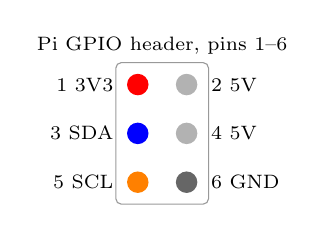
\begin{tikzpicture}[scale=0.62, every node/.style={font=\scriptsize}]
\foreach \r/\a/\b/\ca/\cb in {0/1 3V3/2 5V/red/gray, 1/3 SDA/4 5V/blue/gray, 2/5 SCL/6 GND/orange/black} {
  \fill[\ca] (0,-\r) circle (0.22); \fill[\cb!60] (1,-\r) circle (0.22);
  \node[left] at (-0.3,-\r) {\a}; \node[right] at (1.3,-\r) {\b};
}
\draw[rounded corners=2pt, black!40] (-0.45,0.45) rectangle (1.45,-2.45);
\node at (0.5,0.8) {Pi GPIO header, pins 1--6};
\end{tikzpicture}
\end{minipage}

\smallskip
Which end does your cable have on the Pi side?
\begin{itemize}
\item \textbf{Female sockets:} push straight onto pins 1, 3, 5, 6.
\item \textbf{Male pins:} into the breadboard, four jumpers to the Pi.
\item \textbf{Another JST plug:} solder the breakout's header strip and use four female--female jumpers
  (VIN, GND, SDA, SCL on the breakout's pin row), or use a Pi STEMMA QT adapter.
\end{itemize}
Use pin 1 (3.3\,V), not 5\,V: it keeps the I\textsuperscript{2}C pull-ups at the Pi's logic level.
\begin{lstlisting}
i2cdetect -y 1              # expect "29" in the grid
python3 collect.py check    # live ch0/ch1; Ctrl+C to stop
\end{lstlisting}
\done{\texttt{29} appears, and ch0 drops when you cover the sensor with a finger. Rate $\approx$8\,Hz.}

% ------------------------------------------------------------------
\section{Hole and enclosure \clock{0:30--1:00}}
\begin{center}
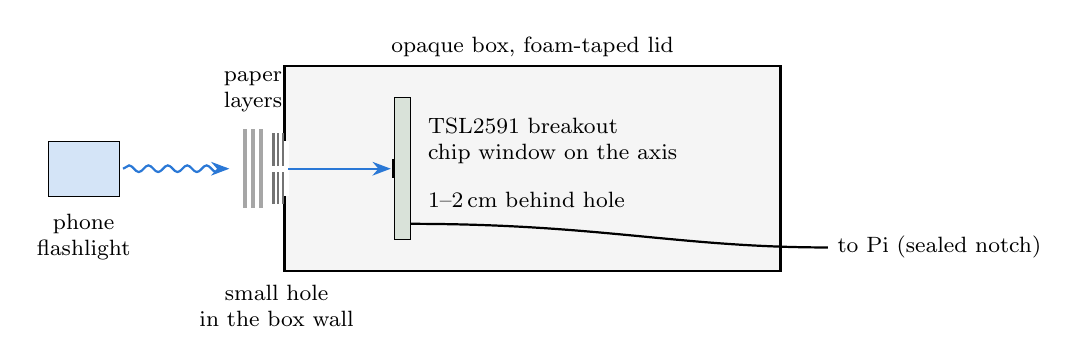
\begin{tikzpicture}[font=\small, >=Stealth]
\draw[thick, fill=black!4] (4,-1.3) rectangle (10.3,1.3);
\node[above, font=\footnotesize] at (7.15,1.3) {opaque box, foam-taped lid};
\draw[line width=3pt, white] (4,-0.35) -- (4,0.35);
\foreach \x in {3.86,3.92,3.98} \draw[line width=0.8pt, black!55] (\x,-0.45) -- (\x,-0.04) (\x,0.04) -- (\x,0.45);
\node[below, font=\footnotesize, align=center] at (3.9,-1.35) {small hole\\in the box wall};
\foreach \x in {3.5,3.6,3.7} \draw[black!35, line width=1.5pt] (\x,-0.5) -- (\x,0.5);
\node[above, font=\footnotesize, align=center] at (3.6,0.6) {paper\\layers};
\draw[fill=accent!20] (1,-0.35) rectangle (1.9,0.35);
\node[below, font=\footnotesize, align=center] at (1.45,-0.45) {phone\\flashlight};
\draw[->, accent, thick, decorate, decoration={snake, amplitude=1.2pt, segment length=7pt}] (1.95,0) -- (3.3,0);
\draw[->, accent, thick] (4.05,0) -- (5.35,0);
\draw[fill=green!25!black!15] (5.4,-0.9) rectangle (5.6,0.9);
\fill[black] (5.36,-0.12) rectangle (5.4,0.12);
\node[right, font=\footnotesize, align=left] at (5.7,0.35) {TSL2591 breakout\\chip window on the axis};
\node[right, font=\footnotesize] at (5.7,-0.4) {1--2\,cm behind hole};
\draw[thick] (5.6,-0.7) .. controls (8,-0.7) and (9,-1) .. (10.9,-1);
\node[right, font=\footnotesize] at (10.9,-1) {to Pi (sealed notch)};
\end{tikzpicture}
\end{center}

\textbf{3a. Hole.} Poke one small hole (pen tip, 2--4\,mm) in a wall of the box. Cut a small notch for the
cable at the lid edge and line the lid seam with foam tape.

\textbf{3b. Mount.} Place the breakout 1--2\,cm behind the hole with the small clear chip facing it, and fix it
with foam tape.

\textbf{3c. Paper.} Tape a few layers of printer paper over the \emph{outside} of the hole. More layers = dimmer.
Change the number of layers if the phone can't get the reading into range.

\textbf{3d. Light source.} Phone flashlight on a stack of books, pointing at the hole. Its \textbf{distance is your
only brightness knob}. Nothing moves during the run.

\textbf{3e. Leak test.} Tape the hole shut with 3 layers of black tape, close the lid, run
\texttt{python3 collect.py check}, then shine the flashlight at every seam and the cable notch.
\done{ch0 sits at a few counts and does not move when you light the seams. If it jumps, add tape or foam where it jumped.}

% ------------------------------------------------------------------
\section{The run \clock{1:00--1:15}}
Remove the black tape from the hole, then:
\begin{lstlisting}
python3 collect.py run          # 5 minutes; --minutes 10 for more random bits
\end{lstlisting}
It shows ch0 live with a hint (\emph{move closer} / \emph{move farther} / \emph{good}). Slide the phone until ch0
is between \textbf{3\,000 and 25\,000}, rest it on the books, press \textbf{Enter}, and don't touch anything until
it finishes. If it never gets bright enough even up close, remove one paper layer.

While it records: open Sonic Pi, paste \texttt{sonic\_pi.rb} into a buffer, press \textbf{Run}; open Overleaf.
\done{\texttt{data/run.csv} saved.}

% ------------------------------------------------------------------
\section{Analyze \clock{1:15--1:20}}
\begin{lstlisting}
python3 analyze.py
\end{lstlisting}
\textbf{How the random numbers are made:} the last bit of each reading (both channels) is a raw coin flip.
A \emph{von Neumann extractor} fixes any bias: read bits in pairs, $01\!\to\!0$, $10\!\to\!1$, throw away
$00$ and $11$. About a quarter of the bits survive. Three clean bits make a number 0--7; keeping only 0--5
gives fair dice.

It prints four randomness tests (pass if $p\ge0.01$), the first 64 bits and 20 dice rolls, and saves
\texttt{data/random\_bits.txt} and \texttt{data/random\_bytes.bin}. It also prints the \textbf{ch0/ch1 noise
correlation}: near 0 means the noise is independent on each photodiode (shot + sensor noise); large means
the phone light is flickering.
\done{all four tests pass. If the noise is under 1.5 counts or tests fail, move the phone closer and redo Step 4.}

% ------------------------------------------------------------------
\section{Sonify and record the demo \clock{1:20--1:50}}
With the Sonic Pi buffer running:
\begin{lstlisting}
python3 sonify.py
\end{lstlisting}
Each 4 debiased noise bits become one bell note (3 bits pick one of 8 notes of A minor pentatonic, 1 bit
picks short or long). Cover the hole: the pad darkens, notes keep coming from the dark noise.
Record 60\,s on your phone showing the box, the terminal and the sound.
\begin{itemize}
\item \textbf{No sound?} Pi 5 has no headphone jack: use HDMI audio or a USB/Bluetooth speaker. In Sonic Pi,
  the Cues panel should show \texttt{/osc:127.0.0.1:\dots/photon/note}.
\item \textbf{Sonic Pi on your laptop instead:} tick ``Allow incoming OSC from other computers'' in its I/O
  settings, then \texttt{python3 sonify.py --host <laptop-ip>}.
\item \textbf{Guaranteed fallback:} \texttt{python3 sonify.py --wav demo.wav} renders 60\,s of music from your
  recorded run, no Sonic Pi needed.
\end{itemize}
\done{you have a demo video (or \texttt{demo.wav}) and a link to it.}

% ------------------------------------------------------------------
\section{Report \clock{1:50--2:30}}
\texttt{analyze.py} already wrote \texttt{report\_overleaf.zip}.
Overleaf $\rightarrow$ New Project $\rightarrow$ Upload Project $\rightarrow$ \texttt{report\_overleaf.zip} $\rightarrow$ Recompile.
Edit the two lines at the top of \texttt{report.tex}: \verb|\authorNames| and \verb|\demoLink|.
Every number, table, figure and verdict sentence comes from your data; the code is in the appendix.
\done{no red ``[run analyze.py]'' placeholders and no red SIMULATED banner. Download the PDF.}

Worth adding in your own words if time allows: one sentence in Discussion naming the light source you used
and anything that went wrong.


% ------------------------------------------------------------------
\section{Extra: math sound waves on the USB speaker \clock{optional, 15 min}}
Plug in the speaker and find its card number, then render and play straight from your recorded run
(no Sonic Pi):
\begin{lstlisting}
aplay -l                                   # e.g. "card 1: USB Audio" -> plughw:1,0
python3 waves.py pluck --device plughw:1,0
python3 waves.py fm    --device plughw:1,0
\end{lstlisting}
Notes come from the same random bits as Step 6; what changes is how each note is synthesized.

\textbf{Pluck (Karplus--Strong string).} A delay line of $N=f_s/f_0$ samples is filled with your
sensor's own standardized noise $z_i=(\Delta x_i-\overline{\Delta x})/\sigma$, then recirculated through
a two-tap averaging filter:
\[
y[n]=\rho\,\tfrac12\bigl(y[n-N]+y[n-N-1]\bigr),\qquad \rho=0.996 .
\]
The averager is a low-pass filter, so high harmonics die first and the noise burst turns into a
decaying plucked string. Every note is excited by a different slice of real measured noise.

\textbf{FM bells.} Frequency modulation with a golden-ratio modulator:
\[
y(t)=e(t)\,\sin\!\bigl(2\pi f_0 t + I(t)\,\sin(2\pi\varphi f_0 t)\bigr),\qquad \varphi=\tfrac{1+\sqrt5}{2}.
\]
The spectrum has sidebands at $f_0\pm k\varphi f_0$ with amplitudes $J_k(I)$ (Bessel functions);
because $\varphi$ is irrational they never line up with harmonics, which sounds like a bell. The
index $I(t)$ is 4$\times$ the rolling mean of $|z|$, so noisier stretches of your data ring brighter.

Both write \texttt{waves\_pluck.wav} / \texttt{waves\_fm.wav}; drop one into your demo video.

% ------------------------------------------------------------------
\section*{Troubleshooting}
\small
\begin{tabularx}{\linewidth}{@{}>{\raggedright\arraybackslash}p{0.33\linewidth} X@{}}
\toprule
Symptom & Fix \\
\midrule
\texttt{i2cdetect} grid empty & I\textsuperscript{2}C not enabled (Step 1), SDA/SCL swapped, loose socket; power-cycle the Pi \\
\texttt{No module named smbus2} & \texttt{sudo apt install -y python3-smbus} \\
\texttt{ID 0x.., expected 0x50} & another chip answers at 0x29; unplug other I\textsuperscript{2}C devices \\
\texttt{TimeoutError} & loose wire; reseat the cable, rerun \\
ch0 stuck near 36\,863 / SATURATED & too much light at MAX gain: more paper, flashlight farther \\
Dark reading moves with room lights & light leak: tape seams, cable notch, hole edges \\
Randomness tests fail & noise too small (move phone closer) or phone moved; record again \\
No notes in Sonic Pi & buffer not running, wrong host, or audio going to the wrong output \\
\texttt{aplay}: silent or wrong speaker & pass \texttt{--device plughw:N,0} with the card number from \texttt{aplay -l} \\
Report shows SIMULATED banner & old simulated data: \texttt{rm -r data}, re-collect, re-analyze \\
\bottomrule
\end{tabularx}

\normalsize
\section*{Files}
\begin{tabularx}{\linewidth}{@{}l X@{}}
\texttt{sensor.py} & TSL2591 driver (one-shot reads so no sample is repeated) + simulator \\
\texttt{collect.py} & \texttt{check}, \texttt{run} \\
\texttt{analyze.py} & random bits, dice, tests, figures, fills the report \\
\texttt{sonify.py}, \texttt{sonic\_pi.rb} & live OSC music / offline WAV \\
\texttt{waves.py} & Karplus--Strong and FM renders played on the USB speaker \\
\texttt{report/report.tex} & the project report (auto-filled) \\
\end{tabularx}

\end{document}
